    % !TEX program = lualatex
\PassOptionsToPackage{naturalnames}{hyperref}
\RequirePackage{luatex85}
\documentclass{article}
\usepackage{geometry}
%\usepackage{fullpage}
\usepackage{parskip}
\usepackage{physics}
\usepackage{amsmath}
\usepackage{amssymb}
\usepackage{xcolor}
\usepackage[colorlinks,linkcolor=blue,citecolor=green]{hyperref}
\usepackage{array}
\usepackage{longtable}
\usepackage{multirow}
\usepackage{comment}
\usepackage{graphicx}
\usepackage{cite}
\usepackage{amsfonts}
\usepackage{bm}
\usepackage{slashed}
\usepackage{dsfont}
\usepackage{mathtools}
\usepackage[compat=1.1.0]{tikz-feynman}
\usepackage{simplewick}
%\usepackage{fourier}
%\usepackage{slashbox}
%\usepackage{intent}
\usepackage{mathrsfs}
\usepackage{xparse}
\usepackage{enumerate}
%\usepackage{axodraw4j}
\usepackage[toc,page]{appendix}
\usepackage{multicol}
\usepackage{authblk}
\usepackage[T1]{fontenc}
%\usepackage{apacite}
%\usepackage{natbib}
%\usepackage[nottoc]{tocbibind}
%\usepackage[backend=biber, style=brent]{biblatex}
%\usepackage[utf8]{inputenc}

%\usepackage{luatexja-fontspec}

\geometry{a4paper,left=2cm,right=2cm}
%\geometry{left=1.3cm,right=1.3cm,top=1.5cm,bottom=2cm}

\newcommand{\gm}{\gamma^{\mu}}
\newcommand{\gn}{\gamma^{\nu}}
\newcommand{\gs}{\gamma^{\sigma}}
\newcommand{\gr}{\gamma^{\rho}}
\newcommand{\gnr}{g^{\nu\rho}}
\newcommand{\gmr}{g^{\mu\rho}}
\newcommand{\gms}{g^{\mu\sigma}}
\newcommand{\gns}{g^{\nu\sigma}}
\newcommand{\vbp}{\vb{p}}
\newcommand{\vbk}{\vb{k}}
\newcommand{\g}{\gamma}
\renewcommand{\a}{\alpha}
\renewcommand{\b}{\beta}
\renewcommand{\t}{\theta}
\newcommand{\la}{\lambda}
\newcommand{\p}{\phi}
\newcommand{\vp}{\varphi}
\newcommand{\s}{\sigma}
\newcommand{\G}{\Gamma}
\newcommand{\pars}{\slashed\partial}
\newcommand{\ps}{\slashed p}
\newcommand{\ks}{\slashed k}
\newcommand{\lag}{\mathcal{L}}
\newcommand{\da}{^{\dagger}}
\newcommand{\sm}{^{\mu}}
\newcommand{\sn}{^{\nu}}
\newcommand{\smn}{^{\mu\nu}}
\newcommand{\Dm}{D^{\mu}}
\newcommand{\dm}{\partial^{\mu}}
\newcommand{\Asquare}{A^{\mu}A_{\mu}}
\newcommand{\partialsquare}[2]{\partial^{\mu}{#1}\partial_{\mu}{#2}}

%\setmainjfont[BoldFont=FandolSong-Bold]{FandolSong-Regular}
%\setsansjfont{FandolSong-Bold}
%\setlength{\parindent}{2em}
%\linespread{1.2}
%\renewcommand\Authsep{, }

\title{Divergence of Klein-Gordon Hydrogen Wavefunction Near Origin}
\author{Yingsheng Huang and Rui Yu}

\begin{document}
\maketitle
\section*{Introduction}
\section{Divergence in Klein-Gordon Equation and Schr\"odinger Equation}
\subsection{Klein-Gordon Equation Solution}
The Klein-Gordon Hydrogen Equation is

\begin{align}
	((i\partial_0+\frac{Z\alpha}{r})^2+\nabla^2-m^2)\Psi=0
\end{align}

For the bound state, the eigen value and the wave function are

\begin{align}
	E    & =m\frac{1}{\sqrt{1+\frac{\alpha^2 Z^2}{(\frac{1}{2}+\sqrt{\frac{1}{4}-Z^2\alpha^2})^2}}} \\
	\Psi & =\frac{c}{\sqrt{4\pi}}e^{-kr}r^\lambda
\end{align}

where

\begin{align}
	\lambda=-\frac{1}{2}+\sqrt{\frac{1}{4}-Z^2\alpha^2}\ \ \ \ \ \
	c=\sqrt{\frac{(2k)^{2(1+\sqrt{\frac{1}{4}-Z^2\alpha^2})}}{\Gamma(2+2\sqrt{\frac{1}{4}-Z^2\alpha^2)})}}\ \ \ \ \ \
	k=\frac{m}{\sqrt{1+\frac{(\frac{1}{2}+\sqrt{\frac{1}{4}-Z^2\alpha^2})^2}{\alpha^2Z^2}}}
\end{align}

c is the normaliztion factor for $\int d^3r|\Psi|^2=1$. For convenience, define

\begin{align}
	\Psi '=\frac{\Psi}{2(mZ\alpha)^\frac{3}{2}}
\end{align}

Now $\Psi '$ is dimensionless and expand it in $\alpha$, we get the origin divergence comes from a term

\begin{align}
	-(Z\alpha)^2\log(m r)
\end{align}

the $m$ in $\log$ could be interpreted as a subtraction point $\mu$.

\subsection{The Schr\"odinger part}

By taking the non-relativistic limit of Klein-Gordon Hydrogen Hamiltonian, the effective Schr\"odinger Hamiltonian is\cite{Holstein2014}

\begin{align}
	H & =H_0+H_{int}                                                                                                                            \\
	H & _0=-\frac{\nabla^2}{2m}-\frac{Z\alpha}{r},\ \ \ H_{int}=\frac{\nabla^4}{8m^3}+\frac{1}{32m^4}[-\nabla^2,[-\nabla^2,-\frac{Z\alpha}{r}]]
\end{align}

The first term of $H_{int}$ is the relativistic kinematic $v^2$ correction, the second one is the Darwin term.\\
The $H_0$ gives the radial wave functions as follows

\begin{align}
	R_{n0} & =\frac{2(mZ\alpha)^\frac{3}{2}}{n^\frac{3}{2}}e^{-\frac{mZ\alpha}{n}r}F(1-n,2,\frac{2mZ\alpha r}{n}),\ \ \ E_n=-\frac{Z^2\alpha^2m}{2n^2}                                \\
	R_{k0} & =\sqrt{\frac{2}{\pi}}(mZ\alpha)^\frac{3}{2}ke^\frac{\pi}{2k}|\Gamma(1-\frac{i}{k})|e^{-imz\alpha kr}F(1+\frac{i}{k},2,2imZ\alpha kr),\ \ \ E_k=\frac{mZ^2\alpha^2k^2}{2}
\end{align}

Within perturbation theory,$E_1^{(1)}=<\phi|H_{int}|\phi>$, in quantum mechanics, the NLO energy correction is

\begin{align}
	E_1^{(1)}=E_1Z^2\alpha^2
\end{align}

The NLO corretion of the bound state wave function is

\begin{align}
	\sum_{n\neq 1}a_{n1}\phi_{n00}+\int dka_{k1}\phi_{k00}
\end{align}

with

\begin{align*}
	a_{n1}=\frac{<\phi_{n00}|H_{int}|\phi_{100}>}{E_1-E_n}=\frac{2 \alpha ^2 \sqrt{n} \left(\left(2 \left(\frac{n-1}{n+1}\right)^n-1\right) n^2+1\right) Z^2}{\left(n^2-1\right)^2}
\end{align*}
and
\begin{align*}
	a_{k1}=\frac{2 \alpha ^4 e^{\frac{\pi }{2 k}} k m^2 Z^4  \abs{\Gamma \left(1-\frac{i}{k}\right)  }\left(\alpha ^2 k^2 m^2 Z^2-2 \alpha ^2 \left(1-\frac{i}{k}\right)^{i/k} \left(1+\frac{i}{k}\right)^{-\frac{i}{k}} m^2 Z^2 \cosh \left(\frac{\pi }{k}\right)+\alpha ^2 m^2 Z^2\right)}{\left(\alpha ^2 k^2 m^2 Z^2+\alpha ^2 m^2 Z^2\right)^2}
\end{align*}

the discrete part of $(12)$ is not divergent at $r=0$. We now focus on the integration part and seperate the relativistic kinematic term and the Darwin term. Since we are only interested in the divergent part, here we give a hard cutoff $\frac{\Lambda}{m}$ as the up-limit of the integration and a also a down-limit $\lambda$, with $\lambda>>1$ (note that the following wave function have been multiplied by $2(mZ\alpha)^\frac{3}{2}$)

\begin{align}
	\Phi^{(1)}(0)_{kin}=\int_\lambda^\frac{\Lambda}{m}dk \frac{2Z^2\alpha^2k^\frac{3}{2}}{2\pi(\sqrt{1-\exp(-\frac{2 \pi}{k})})}(1-\frac{2}{1+k^2}\exp(-\frac{2\arctan(k)}{k}))e^\frac{\pi}{2k}|\Gamma(1-\frac{i}{k})|
\end{align}

with the integral region we defined$(k\ll1)$, it would be OK to expand the integrand in $\frac{1}{k}$ (I havn't prove it yet), then the UV divergent term is

\begin{align}
	\Phi^{(1)}(0)_{kin} & =\int_\lambda^\frac{\Lambda}{m}dk(Z\alpha)^2(\frac{1}{\pi}+\frac{1}{k}) \\
	                    & \sim(\alpha Z)^2(\frac{\Lambda}{\pi m}+\log(\frac{\Lambda}{m}))
\end{align}

The UV divergent part of Darwin term is
\begin{align}
	\Phi^{(1)}(0)_D=-\frac{(Z\alpha)^4}{8\pi}\int_\lambda^\frac{\Lambda}{m}dkk^2e^\frac{\pi}{k}|\Gamma(1-\frac{i}{k})|^2
\end{align}

with the same trick as $(15)$, the UV divergen part is

\begin{align}
	\Phi^{(1)}(0)_{D} & =-(\alpha Z)^4\int_\lambda^\frac{\Lambda}{m}dk\frac{k^2}{8\pi}+\frac{k}{8}+\frac{1}{24}\pi               \\
	                  & \sim -\frac{(Z\alpha)^4}{8\pi}(\frac{\Lambda^3}{3m^3}+\frac{\pi\Lambda^2}{2m^2}+\frac{\pi^2\Lambda}{3m})
\end{align}

Now collect all the results we get as follows.\\
The K-G wave function's origin UV divergence is

\begin{align}
	K-G\ \ UV & :-(Z\alpha)^2\log(m r)
\end{align}

The purterbative Schr\"odinger wave function's origin UV divergence, with a k cutoff $\frac{\Lambda}{m}$, is

\begin{align}
	Kin\ \  UV    & :(\alpha Z)^2(\frac{\Lambda}{\pi m}+\log(\frac{\Lambda}{m}))                                         \\
	Darwin\ \  UV & :-\frac{(Z\alpha)^4}{8\pi}(\frac{\Lambda^3}{3m^3}+\frac{\pi\Lambda^2}{2m^2}+\frac{\pi^2\Lambda}{3m})
\end{align}

All the $m$, under $\Lambda$ or in a $\log$, can be interpreted as a subtraction point $\mu$.

\section{Non-relativistic Scalar QED (NRSQED) Matching}
\subsection{Operator Product Expansion}
In the following sections we work on the quantum field theory side. Assuming the full theory of the scalar electron is scalar QED, we can mimic the effect of neucleus, or rather to say, Coulomb potential, with heavy scalar effective theory. For simplicity, there's no need involving any other effect the nucleus might have. Therefore, we can describe the wavefunction in terms of a matrix element $\mel{0}{\psi(x)N(0)}{0}$. The divergence of this non-local matrix element can be analyzed by operator product expansion\cite{Lepage:1997cs}.

The operator product expansion\cite{Collins1984} (OPE) is to write the products of several local operators evaluated at different points, in the limit of those points approaching each other, as a series of composite local operators, i.e.
\begin{align}
	\mathcal{O}_1(x)\mathcal{O}_2(y)=\sum_nC_n(x-y)\mathcal{O}_n(x)
\end{align}
In our case, the equation becomes
\begin{align}
	\mel{0}{\psi(x)N(0)}{0}=\mel{0}{C_0(x)\psi(0)N(0)+\sum_nC_n(x)\mathcal{O}_n(0)}{0}\label{OPE}
\end{align}
The logarithmic divergence, which is the highest order of divergence on the left hand side, only appears in the first term of the right hand side.

Intuitively, we can assume $\psi(x)$ is just the scalar field operator in scalar QED. But what we need is logarithmic divergence start at $Z^2\a^2$ order, and using relativistic scalar field operator will result in logarithmic divergence at $Z\a$ order, which, since we already know the answer to the question, is not what we want. However, since QED, or in our case, scalar QED, has no bound on how small the distance it can probe, we might observe that in order to investigate low energy physics, we can't use theory with such sensitivity in short range.

The alternative is to use non-relativistic scalar QED on the scalar electron side. Through it's a non-relativistic theory thus not the first chioce when studying a relativistic problem, the natural energy cutoff it provides will be very convenient in this problem.
\subsection{Feynman Rules}
\subsubsection{Scalar QED (SQED)}
The Lagrangian of scalar QED is
\begin{align}
	\lag_{SQED}=\abs{D_{\mu}\phi}^2-m^2\abs{\phi}^2+\Phi_v^*iv\cdot D\Phi_v
	\label{SQEDLAG}
\end{align}
with the covariant derivative defined as
\begin{align*}
	D_{\mu}\phi=\partial_{\mu}\phi+ieA_{\mu}\phi
\end{align*}
and
\begin{align*}
	D_{\mu}\Phi_v=\partial_{\mu}\Phi-iZeA_{\mu}\Phi_v
\end{align*}
But note that no dynamic electromagnetic field $\vb{A}$ can appear in actual calculation because here only static scalar potential exists.

And the Feynman rules are
%\clearpage
\begin{multicols}{2}
	\begin{align*}
		\feynmandiagram[small,horizontal=a to b]{
		a -- [momentum=\(p\)] b,
		}; & =\frac{i}{p^2-m^2+i\epsilon} \\
		\feynmandiagram[small,horizontal=a to o,baseline=(o.base)]{
		a -- [momentum=\(p_1\)] o,
		o -- [momentum=$p_2$] b,
		c -- [photon] o,
		}; & =-ie(p_1^{\mu}+p_2^{\mu})    \\
		\feynmandiagram[small,horizontal=a to b,baseline=(o.base)]{
		a -- [momentum'=$p_1$] o -- [momentum'=$p_2$] b,
		c -- [photon] o,
		d -- [photon] o,
		}; & =2ie^2g^{\mu\nu}
	\end{align*}
	\begin{align*}
		\feynmandiagram[small,horizontal=a to b]{
		a -- [momentum=$mv+k$,double distance=1pt] b,
		}; & =\frac{i}{v\cdot k} \\
		\feynmandiagram[small,baseline=(o.base)]{
		a -- [double distance=1pt] o -- [double distance=1pt] b,
		c -- [photon] o,
		}; & =iZev^{\mu}         \\\\\\
		\feynmandiagram[small,horizontal=a to b]{
		a [particle=$A^0$] -- [photon,momentum=$q$] b,
		}; & =\frac{i}{\vb{q}^2}
	\end{align*}
\end{multicols}
\subsubsection{NRSQED}
Using the transformation $\displaystyle\phi\rightarrow\frac{e^{-imt}}{\sqrt{2m}}\varphi$, we can have the Lagrangian
\begin{align}
	\lag_{NRSQED}=\varphi^*\pqty{iD_0+\frac{\vb{D}^2}{2m}}\varphi+\delta\lag +\Phi_v^*iv\cdot D\Phi_v
	\label{NRSQEDLAG}
\end{align}
with the same notation above. Here $\vb{D}=\nabla-ie\vb{A}$.

Feynman rules are also the same except for the scalar electron side which becomes
\begin{align*}
	\feynmandiagram[small,horizontal=a to b]{
	a -- [momentum=$p$] b,
	};=\frac{i}{E-\frac{\vb{p}^2}{2m}+i\epsilon}\;\;\;\;\;\;\;\;\;\;\;\;\;\;\;
	\feynmandiagram[small,horizontal=a to o,baseline=(o.base)]{
	a -- [momentum=$p_1$] o,
	o -- [momentum=$p_2$] b,
	c [particle=$A^0$] -- [photon] o,
	};=-ie
\end{align*}
We can ignore all interacting terms involving $\vb{A}$.

Since we need to match it to $\mathcal{O}(v^2)$ order
\begin{align}
	\delta\lag=\frac{(D_0\varphi)^*(D_0\varphi)}{2m}=\frac{\dot{\varphi}^*\dot{\varphi}}{2m}+\frac{e^2\varphi^*\varphi A_0^2}{2m}-\frac{ie}{2m}A_0(\varphi^*\dot{\varphi}-\dot{\varphi}^*\varphi)
	\label{deltaLAG}
\end{align}
and it changes the Feynman rules to\footnote{In this note, $p^0$ is the zero component of relativistic four momentum, and $E=p^0-m$. }
\begin{align*}
	\feynmandiagram[small,horizontal=a to o,baseline=(o.base)]{
	a -- [momentum=$p_1$] o,
	o -- [momentum=$p_2$] b,
	c [particle=$A^0$] -- [photon] o,
	};=-ie(1+\frac{E_1+E_2}{2m})\;\;\;\;\;
	\feynmandiagram[small,horizontal=a to b,baseline=(o.base)]{
	a -- [momentum'=$p_1$] o -- [momentum'=$p_2$] b,
	c [particle=$A^0$] -- [photon] o,
	d [particle=$A^0$] -- [photon] o,
	}; & =\frac{ie^2}{2m}
\end{align*}

Since we rescaled $\phi$ by $\frac{1}{\sqrt{2m}}$ to get $\varphi$, the in/out states are also changed. We must multiply them by $\sqrt{2p^0}$ to compensate that change.

Another way to achieve it is to use the transform rules of heavy scalar effective theory (HSET). \subsubsection{NRSQED Lagrangian via HSET transformation}
Let's focus on the lagrangian of only a single Scalar field
\begin{align}
	\lag_{SQED}=\abs{D_{\mu}\phi}^2-m^2\abs{\phi}^2
\end{align}
Substitute $\phi$ for $\phi=\frac{1}{\sqrt{2m}}e^{-imv\cdot x}(\varphi_v+\bar{\varphi}_v)$ with (Schwartz, Sec 35.2)
\begin{align}
	\varphi_v       & =\frac{1}{\sqrt{2m}}e^{imv\cdot x}(iv\cdot D+m)\phi  \\
	\bar{\varphi}_v & =\frac{1}{\sqrt{2m}}e^{imv\cdot x}(-iv\cdot D+m)\phi
\end{align}
then
\begin{align}
	\lag_{SQED}=\frac{1}{2m}(D_\mu(\varphi_v+\bar{\varphi}_v))^*D^\mu(\varphi_v+\bar{\varphi}_v)+(\varphi_v+\bar{\varphi}_v)^*iv\cdot D(\varphi+\bar{\varphi}_v)
\end{align}
Within our calculation, we set $\vec{A}=0,v=(1,\vec{0})$. Then from $(25),(26)$ and the motion equation derived from $(27)$, we get two equation
\begin{align}
	\bar{\varphi}_v           & =\frac{-iD_0}{2m}(\varphi_v+\bar{\varphi}_v)      \\
	\frac{-iD_0}{2m}\varphi_v & =\frac{\nabla^2}{4m^2}(\varphi_v+\bar{\varphi}_v)
\end{align}
And $(27)$ could be transformed as
\begin{align}
	\lag_{SQED}=(\varphi_v+\bar{\varphi}_v)^*(iD_0+\frac{\nabla^2}{2m}-\frac{D_0^2}{2m})(\varphi+\bar{\varphi}_v)
\end{align}
Substituting $(28),(29)$ iteratively, then we get the $\lag$ expanding for $v$ as
\begin{align}
	\lag_{SQED}=\varphi_v^*(iD_0+\frac{\nabla^2}{2m}+\frac{\nabla^4}{8m^3}+\frac{\nabla^6}{16m^5}+\frac{e}{32m^4}([\nabla^2,[A_0,\nabla^2]]+[A_0,\nabla^4])+\mathcal{O}(v^7))\varphi_v
\end{align}


\subsection{LO Matching}
\subsubsection{SQED}
\begin{align*}
	i\mathcal{M}_{SQED}^{(0)} & =\feynmandiagram[horizontal=i1 to f1,layered layout,inline=($(a)!0.5!(c)$),small]{
	i1[particle=$P_N$] -- [double distance=1pt] a -- [double distance=1pt] f1[particle=$P_N$],
	i2[particle=$p_1$] -- [] c -- [] f2[particle=$p_2$],
	{ [same layer] a -- [photon,momentum'=$q$] c},
	};=-e^2v^{0}\frac{i(p_1^0+p_2^0)}{\vb{q}^2}=-e^2v^0\frac{i}{\vb{q}^2}(2m+2E_1)
\end{align*}
\subsubsection{NRSQED}
\begin{align*}
	i\mathcal{M}_{NRSQED}^{(0)} & =\feynmandiagram[horizontal=i1 to f1,layered layout,inline=($(a)!0.5!(c)$),small]{
	i1[particle=$P_N$] -- [double distance=1pt] a -- [double distance=1pt] f1[particle=$P_N$],
	i2[particle=$p_1$] -- [] c -- [] f2[particle=$p_2$],
	{ [same layer] a -- [photon,momentum'=$q$] c},
	};=-2\sqrt{p^0_1p^0_2}e^2v^{0}\frac{i(1+\delta)}{\vb{q}^2}=-e^2v^0\times 2p_1^0\frac{i(1+\delta)}{\vb{q}^2}
\end{align*}
which gives
\begin{align*}
	\delta=\frac{p_1^0+p_2^0}{2\sqrt{p_1^0p_2^0}i}-1\approx \frac{\vb{p}_1^4-2 \vb{p}_1^2 \vb{p}_2^2+\vb{p}_2^4}{32 m^4}
\end{align*}
The extra electron-photon vertex is
\begin{align*}
	\feynmandiagram[small,horizontal=a to o,baseline=(o.base)]{
	a -- [momentum=$p_1$] o [dot],
	o -- [momentum=$p_2$] b,
	c [particle=$A^0$] -- [photon] o,
	}; & =-i\frac{\vb{p}_1^4-2 \vb{p}_1^2 \vb{p}_2^2+\vb{p}_2^4}{32 m^4}
\end{align*}
We can write the correction interacting term corresponding to $\delta$ as
\begin{align*}
	A_0\varphi\nabla^4\varphi^*-2A_0\nabla^2\varphi^*\nabla^2\varphi+\varphi^*A_0\nabla^4\varphi
	  & =\varphi^*\nabla^4(A_0\varphi)-2\varphi^*\nabla^2(A_0\nabla^2\varphi)+\varphi^*A_0\nabla^4\varphi \\
	  & =\varphi^*(\nabla^2[\nabla^2,A_0]-[\nabla^2,A_0]\nabla^2)\varphi                                  \\
	  & =\varphi^*[\nabla^2,[\nabla^2,A_0]]\varphi
\end{align*}
which is exactly the Darwin term in Holstein's \emph{Advanced Topics in QM} with coefficient $1/32m^4$.
  
\iffalse\subsection{NLO}
\subsubsection{SQED}
\begin{align*}
	i\mathcal{M}_{SQED}^{(1)} & =\feynmandiagram[horizontal=i1 to f1,layered layout,inline=($(a)!0.5!(c)$),medium]{
	i1[particle=$P_N$] -- [double distance=1pt] a -- [double distance=1pt,momentum=$P_N-k^0$] b -- [double distance=1pt] f1[particle=$P_N$],
	i2[particle=$p_1$] -- [] c -- [momentum=$p_1+k$] d -- [] f2[particle=$p_2$],
	{ [same layer] a -- [photon,momentum'=$k$] c},
	{ [same layer] b -- [photon,rmomentum=$k-q$] d},
	};
	+
	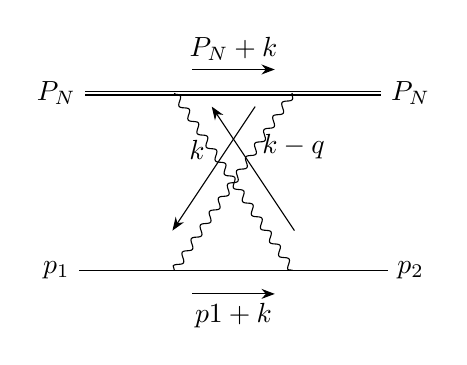
\begin{tikzpicture}[baseline=($(a)!0.5!(c)$)]
		\begin{feynman}
			\diagram[horizontal=i1 to f1,layered layout,medium]{
			i1[particle=$P_N$] -- [double distance=1pt] a -- [double distance=1pt,momentum=$P_N+k$] b -- [double distance=1pt] f1[particle=$P_N$],
			i2[particle=$p_1$] -- [] c -- [momentum'=$p1+k$] d -- [] f2[particle=$p_2$],
			{ [same layer] a --[draw=none] c},
			{ [same layer] b-- [draw=none] d},
			};
			\diagram*{
			(a) -- [photon,rmomentum=$k-q$] (d),
			(b) -- [photon,momentum'=$k$] (c),
			};
		\end{feynman}
	\end{tikzpicture}
	+
	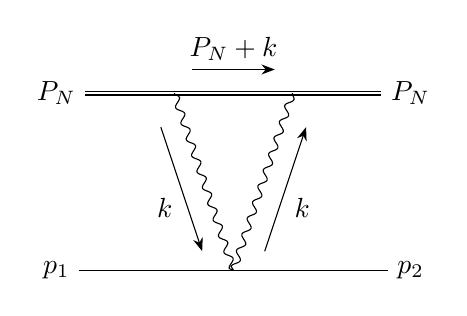
\begin{tikzpicture}[baseline=($(a)!0.5!(c)$)]
		\begin{feynman}
			\diagram[horizontal=i1 to f1,layered layout,medium]{
			i1[particle=$P_N$] -- [double distance=1pt] a -- [double distance=1pt,momentum=$P_N+k$] b -- [double distance=1pt] f1[particle=$P_N$],
			i2[particle=$p_1$] -- [] c -- [] d -- [] f2[particle=$p_2$],
			{ [same layer] a --[draw=none] c},
			{ [same layer] b-- [draw=none] d},
			};
			\vertex at ($(c)!0.5!(d)$) (f);
			\diagram*{
			(a) -- [photon,momentum'=$k$] (f),
			(b) -- [photon,rmomentum=$k$] (f),
			};
		\end{feynman}
	\end{tikzpicture}
\end{align*}
\begin{align*}
	\feynmandiagram[horizontal=i1 to f1,layered layout,inline=($(a)!0.5!(c)$),medium]{
	i1[particle=$P_N$] -- [double distance=1pt] a -- [double distance=1pt,momentum=$P_N-k^0$] b -- [double distance=1pt] f1[particle=$P_N$],
	i2[particle=$p_1$] -- [] c -- [momentum=$p_1+k$] d -- [] f2[particle=$p_2$],
	{ [same layer] a -- [photon,momentum'=$k$] c},
	{ [same layer] b -- [photon,rmomentum=$k-q$] d},
	};=-e^2v^{0}\int\frac{\dd^4k}{(2\pi)^4}\frac{i}{\vb{k}^2}\frac{}{}<+content+>
\end{align*}<++>
\begin{align*}
	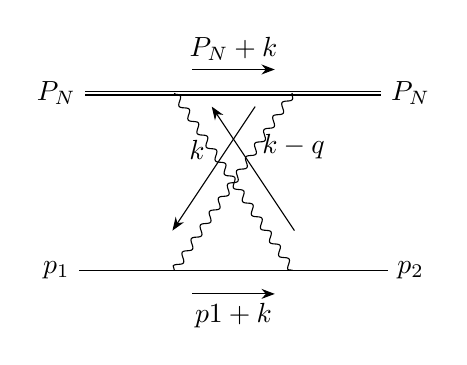
\begin{tikzpicture}[baseline=($(a)!0.5!(c)$)]
		\begin{feynman}
			\diagram[horizontal=i1 to f1,layered layout,medium]{
			i1[particle=$P_N$] -- [double distance=1pt] a -- [double distance=1pt,momentum=$P_N+k$] b -- [double distance=1pt] f1[particle=$P_N$],
			i2[particle=$p_1$] -- [] c -- [momentum'=$p1+k$] d -- [] f2[particle=$p_2$],
			{ [same layer] a --[draw=none] c},
			{ [same layer] b-- [draw=none] d},
			};
			\diagram*{
			(a) -- [photon,rmomentum=$k-q$] (d),
			(b) -- [photon,momentum'=$k$] (c),
			};
		\end{feynman}
	\end{tikzpicture} <+content+>
\end{align*}<++>
\begin{align*}
	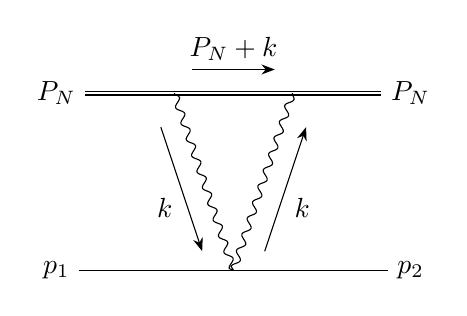
\begin{tikzpicture}[baseline=($(a)!0.5!(c)$)]
		\begin{feynman}
			\diagram[horizontal=i1 to f1,layered layout,medium]{
			i1[particle=$P_N$] -- [double distance=1pt] a -- [double distance=1pt,momentum=$P_N+k$] b -- [double distance=1pt] f1[particle=$P_N$],
			i2[particle=$p_1$] -- [] c -- [] d -- [] f2[particle=$p_2$],
			{ [same layer] a --[draw=none] c},
			{ [same layer] b-- [draw=none] d},
			};
			\vertex at ($(c)!0.5!(d)$) (f);
			\diagram*{
			(a) -- [photon,momentum'=$k$] (f),
			(b) -- [photon,rmomentum=$k$] (f),
			};
		\end{feynman}
	\end{tikzpicture}<+content+>
\end{align*}<++>
\subsubsection{NRSQED}\fi

\section{Local Operator and Matrix Element of NRSQED}
To reproduce the singular behavior of ``Klein-Gordon Hydrogen'' wavefunction near origin, we can try OPE. But the dependence of x in OPE can be taken as a regularization scheme and thus the result should be the same as local one without renormalization. And the logarithmic terms of x in OPE can be reproduced by the logarithmic divergence of local operators. Since in the study of Klein-Gordon equation we know that the wavefunction only contains logarithmic divergence at the origin so that's the only type of divergence we're looking for.
\subsection{NLO}
It's obvious that the tree level has no divergence of any kind, so we'll start at one loop. 

First we define $\epsilon=3-d$. After dimensional regularization, the Gamma function in the numerator is something like $\Gamma(n-d/2)$ and Gamma function doesn't have pole at half integer. We can prove that any one-loop diagram involved does not have logarithmic divergence, for example
\begin{align*}
	  & \mel{0}{\psi_e(0)N(0)(-ie\mu^{-\epsilon})\int\dd^4y\bar\psi_e\psi_e A^0(-iZe\mu^{-\epsilon})\int\dd^4z\bar NNA^0}{eN}=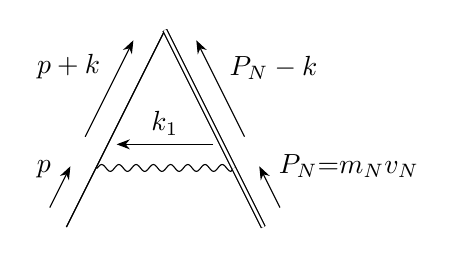
\begin{tikzpicture}[baseline=($(p1)!0.5!(x)$)]
		\begin{feynman}
			\vertex (p1);
			\vertex[right=2.5cm of p1] (p2);
			\vertex at ($(p1)!0.5!(p2)+(0,2.5cm)$) (x) ;
			\vertex at ($(p1)!0.3!(x)$) (y1);
			\vertex at ($(p2)!0.3!(x)$) (z1);
			%
			\diagram* {
			(p1) -- [] (x);
			(p2) -- [double distance=1pt] (x);
			(y1) -- [photon,rmomentum=$k_1$] (z1);
			(p1) -- [momentum=\(p\)] (y1);
			(p2) -- [momentum'=$P_{N}\text{=}m_{N}v_{N}$,double distance=1pt] (z1);
			(y1) -- [momentum=\(p+k\)] (x);
			(z1) -- [momentum'=\(P_{N}-k\),double distance=1pt] (x);
			};
		\end{feynman}
	\end{tikzpicture}
\end{align*}
which doesn't have logarithm divergence.
\subsection{NNLO}
\begin{align*}
	&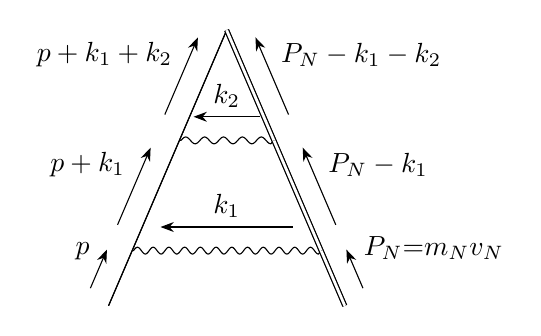
\begin{tikzpicture}[baseline=($(p1)!0.5!(x)$)]
		\begin{feynman}
			\vertex (p1);
			\vertex[right=3cm of p1] (p2);
			\vertex at ($(p1)!0.5!(p2)+(0,3.5cm)$) (x) ;
			\vertex at ($(p1)!0.2!(x)$) (y1);
			\vertex at ($(p2)!0.2!(x)$) (z1);
			\vertex at ($(p1)!0.6!(x)$) (y2);
			\vertex at ($(p2)!0.6!(x)$) (z2);
			%
			\diagram* {
			(p1) -- [] (x);
			(p2) -- [double distance=1pt] (x);
			(y1) -- [photon,rmomentum=$k_1$] (z1);
			(y2) -- [photon,rmomentum=$k_2$] (z2);
			(p1) -- [momentum=\(p\)] (y1);
			(p2) -- [momentum'=$P_{N}\text{=}m_{N}v_{N}$,double distance=1pt] (z1);
			(y1) -- [momentum=\(p+k_1\)] (y2);
			(z1) -- [momentum'=\(P_{N}-k_1\),double distance=1pt] (z2);
			(y2) -- [momentum=\(p+k_1+k_2\)] (x);
			(z2) -- [momentum'=\(P_{N}-k_1-k_2\),double distance=1pt] (x);
			};
		\end{feynman}
	\end{tikzpicture}\\ =&-\mu^{2\epsilon}Z^2e^4\bqty{\int[dk_1][dk_2]\frac{1}{\vb{\abs{k_1}}^2}\frac{1}{\vb{\abs{k_2}}^2}\frac{1}{-k_1^0-k_2^0+i\epsilon}\frac{1}{-k_1^0+i\epsilon}\frac{1}{E+k_1^0-\frac{\vb{(p+k_1)}^2}{2m}+i\epsilon}\frac{1}{E+k_1^0+k_2^0-\frac{\vb{(p+k_1+k_2)}^2}{2m}+i\epsilon}}
	\\
	\intertext{integrate out the temporal component of loop momentum, then perform a shift on them}
	=&\mu^{2\epsilon}Z^2e^4\bqty{\int\frac{\dd^3\vb{k_1}}{(2\pi)^3}\frac{\dd^3\vb{k_2}}{(2\pi)^3}\frac{1}{\vb{\abs{k_1-p}}^2}\frac{1}{\vb{\abs{k_2-k_1}}^2}\frac{1}{E-\frac{\vb{\abs{k_1}}^2}{2m}+2i\epsilon}\frac{1}{E-\frac{\vb{\abs{k_2}}^2}{2m}+2i\epsilon}}=\text{finite terms}
\end{align*}
\begin{align*}
	  & 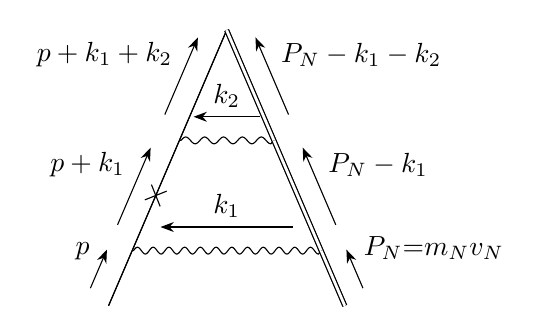
\begin{tikzpicture}[baseline=($(p1)!0.5!(x)$)]
		\begin{feynman}
			\vertex (p1);
			\vertex[right=3cm of p1] (p2);
			\vertex at ($(p1)!0.5!(p2)+(0,3.5cm)$) (x) ;
			\vertex at ($(p1)!0.2!(x)$) (y1);
			\vertex at ($(p2)!0.2!(x)$) (z1);
			\vertex at ($(p1)!0.6!(x)$) (y2);
			\vertex at ($(p2)!0.6!(x)$) (z2);
			\vertex at ($(y1)!0.5!(z1)$) (t);
			%
			\diagram* {
			(p1) -- [] (x);
			(p2) -- [double distance=1pt] (x);
			(y1) -- [photon,rmomentum=$k_1$] (z1);
			(y2) -- [photon,rmomentum=$k_2$] (z2);
			(p1) -- [momentum=\(p\)] (y1);
			(p2) -- [momentum'=$P_{N}\text{=}m_{N}v_{N}$,double distance=1pt] (z1);
			(y1) -- [momentum=\(p+k_1\),insertion=0.5] (y2);
			(z1) -- [momentum'=\(P_{N}-k_1\),double distance=1pt] (z2);
			(y2) -- [momentum=\(p+k_1+k_2\)] (x);
			(z2) -- [momentum'=\(P_{N}-k_1-k_2\),double distance=1pt] (x);
			};
		\end{feynman}
	\end{tikzpicture}=4m^2\mu^{2\epsilon}Z^2e^4
	\int\frac{\dd^3\vb{k_1}}{(2\pi)^3}\frac{\dd^3\vb{k_2}}{(2\pi)^3}\frac{1}{\vb{\abs{k_1-p}}^2}\frac{1}{\vb{\abs{k_2-k_1}}^2}\frac{\vb{\abs{k_1}}^4/4m^2}{[\vb{\abs{k_1}}^2-2mE]^2}\frac{1}{\vb{\abs{k_2}}^2-2mE}\\
	= & Z^2\a^2(\frac{1}{2(3-d)}+\log \mu)+\text{finite terms}
\end{align*}
\begin{align*}
	  & 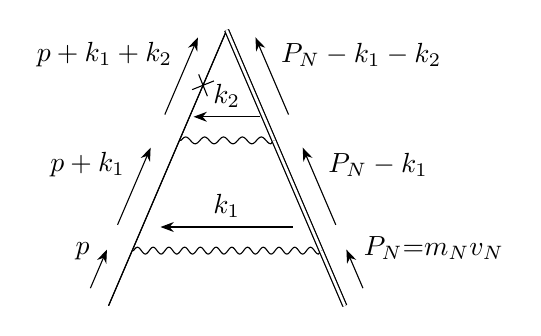
\begin{tikzpicture}[baseline=($(p1)!0.5!(x)$)]
		\begin{feynman}
			\vertex (p1);
			\vertex[right=3cm of p1] (p2);
			\vertex at ($(p1)!0.5!(p2)+(0,3.5cm)$) (x) ;
			\vertex at ($(p1)!0.2!(x)$) (y1);
			\vertex at ($(p2)!0.2!(x)$) (z1);
			\vertex at ($(p1)!0.6!(x)$) (y2);
			\vertex at ($(p2)!0.6!(x)$) (z2);
			\vertex at ($(y1)!0.5!(z1)$) (t);
			%
			\diagram* {
			(p1) -- [] (x);
			(p2) -- [double distance=1pt] (x);
			(y1) -- [photon,rmomentum=$k_1$] (z1);
			(y2) -- [photon,rmomentum=$k_2$] (z2);
			(p1) -- [momentum=\(p\)] (y1);
			(p2) -- [momentum'=$P_{N}\text{=}m_{N}v_{N}$,double distance=1pt] (z1);
			(y1) -- [momentum=\(p+k_1\)] (y2);
			(z1) -- [momentum'=\(P_{N}-k_1\),double distance=1pt] (z2);
			(y2) -- [momentum=\(p+k_1+k_2\),insertion=0.5] (x);
			(z2) -- [momentum'=\(P_{N}-k_1-k_2\),double distance=1pt] (x);
			};
		\end{feynman}
	\end{tikzpicture}=4m^2
	\mu^{2\epsilon}Z^2e^4\int\frac{\dd^3\vb{k_1}}{(2\pi)^3}\frac{\dd^3\vb{k_2}}{(2\pi)^3}\frac{1}{\vb{\abs{k_1-p}}^2}\frac{1}{\vb{\abs{k_2-k_1}}^2}\frac{1}{\vb{\abs{k_1}}^2-2mE}\frac{\vb{\abs{k_2}}^4/4m^2}{[\vb{\abs{k_2}}^2-2mE]^2}\\
	= & 0+\text{finite terms}
\end{align*}
we can see that the total divergence is $Z^2\a^2(\frac{1}{2(3-d)}+\log \mu)$.

Comparing the final result of divergence between OPE and QM wavefunctions, we can see that the coefficient of $\log{\mu}$ is consistent with which of the logarithm divergence in the asymptotic behavior of Klein-Gordon wavefunction and Schr\"odinger wavefunction with relativistic correction.

\section{Operator Product Expansion and Explicitly Coordinate-dependent Divergence}
Now that we have successfully isolated the logarithmic divergence of local operators, we can calculate the coordinate-dependent divergence that we actually encountered regarding the wavefunction. For any type of diagrams on the left hand side of equation \eqref{OPE}, we have
\begin{align}
	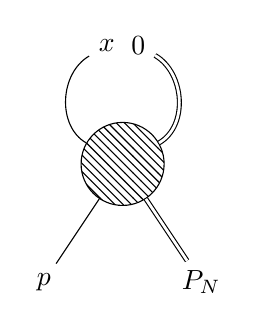
\begin{tikzpicture}[baseline=($(p1)!0.5!(x)$)]
		\tikzfeynmanset{
			my blob/.style={
					/tikzfeynman/blob,
					/tikz/minimum size=30pt,
				},
			%every vertex/.style={my blob},
		}
		\begin{feynman}
			\vertex (p1) {$p$};
			\vertex[right=2cm of p1] (p2) {$P_N$};
			\vertex at ($(p1)!0.4!(p2)+(0,3cm)$) (x) {$x$};
			\vertex at ($(p1)!0.6!(p2)+(0,3cm)$) (0) {$0$};
			\vertex at ($(p1)!0.5!(x)$) (y1);
			\vertex at ($(p2)!0.5!(0)$) (z1);
			\vertex at ($(y1)!0.5!(z1)$) (o);
			\node[my blob] at (o) (o1);
			%
			\diagram* {
			(p1) --  (o1);
			(p2) -- [double distance=1pt] (o1);
			%(y1) -- [photon,rmomentum=$k_1$] (z1);
			%(p1) -- [] (y1);
			%(p2) -- [double distance=1pt] (z1);
			(o1) -- [out=150, in=210] (x);
			(o1) -- [out=30, in=330,double distance=1pt] (0);
			};
		\end{feynman}
	\end{tikzpicture}
	=
	\bqty{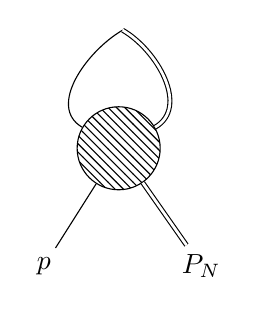
\begin{tikzpicture}[baseline=($(p1)!0.5!(x)$)]
		\tikzfeynmanset{
			my blob/.style={
					/tikzfeynman/blob,
					/tikz/minimum size=30pt,
				},
			%every vertex/.style={my blob},
		}
		\begin{feynman}
			\vertex (p1) {$p$};
			\vertex[right=2cm of p1] (p2) {$P_N$};
			\vertex at ($(p1)!0.4!(p2)+(0,3cm)$) (x) ;
			\vertex at ($(p1)!0.5!(p2)+(0,3cm)$) (0) ;
			\vertex at ($(p1)!0.5!(x)$) (y1);
			\vertex at ($(p2)!0.5!(0)$) (z1);
			\vertex at ($(y1)!0.5!(z1)$) (o);
			\node[my blob] at (o) (o1);
			%
			\diagram* {
			(p1) --  (o1);
			(p2) -- [double distance=1pt] (o1);
			%(y1) -- [photon,rmomentum=$k_1$] (z1);
			%(p1) -- [] (y1);
			%(p2) -- [double distance=1pt] (z1);
			(o1) -- [out=150, in=210] (0);
			(o1) -- [out=30, in=330,double distance=1pt] (0);
			};
		\end{feynman}
	\end{tikzpicture}-UV}
	+
	\bqty{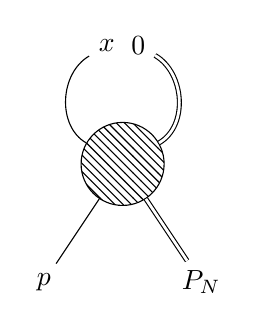
\begin{tikzpicture}[baseline=($(p1)!0.5!(x)$)]
		\tikzfeynmanset{
			my blob/.style={
					/tikzfeynman/blob,
					/tikz/minimum size=30pt,
				},
			%every vertex/.style={my blob},
		}
		\begin{feynman}
			\vertex (p1) {$p$};
			\vertex[right=2cm of p1] (p2) {$P_N$};
			\vertex at ($(p1)!0.4!(p2)+(0,3cm)$) (x) {$x$};
			\vertex at ($(p1)!0.6!(p2)+(0,3cm)$) (0) {$0$};
			\vertex at ($(p1)!0.5!(x)$) (y1);
			\vertex at ($(p2)!0.5!(0)$) (z1);
			\vertex at ($(y1)!0.5!(z1)$) (o);
			\node[my blob] at (o) (o1);
			%
			\diagram* {
			(p1) --  (o1);
			(p2) -- [double distance=1pt] (o1);
			%(y1) -- [photon,rmomentum=$k_1$] (z1);
			%(p1) -- [] (y1);
			%(p2) -- [double distance=1pt] (z1);
			(o1) -- [out=150, in=210] (x);
			(o1) -- [out=30, in=330,double distance=1pt] (0);
			};
		\end{feynman}
	\end{tikzpicture}-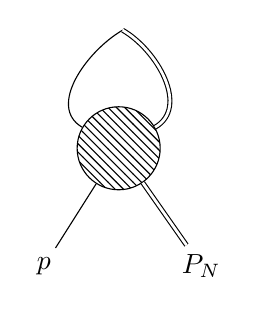
\begin{tikzpicture}[baseline=($(p1)!0.5!(x)$)]
		\tikzfeynmanset{
			my blob/.style={
					/tikzfeynman/blob,
					/tikz/minimum size=30pt,
				},
			%every vertex/.style={my blob},
		}
		\begin{feynman}
			\vertex (p1) {$p$};
			\vertex[right=2cm of p1] (p2) {$P_N$};
			\vertex at ($(p1)!0.4!(p2)+(0,3cm)$) (x) ;
			\vertex at ($(p1)!0.5!(p2)+(0,3cm)$) (0) ;
			\vertex at ($(p1)!0.5!(x)$) (y1);
			\vertex at ($(p2)!0.5!(0)$) (z1);
			\vertex at ($(y1)!0.5!(z1)$) (o);
			\node[my blob] at (o) (o1);
			%
			\diagram* {
			(p1) --  (o1);
			(p2) -- [double distance=1pt] (o1);
			%(y1) -- [photon,rmomentum=$k_1$] (z1);
			%(p1) -- [] (y1);
			%(p2) -- [double distance=1pt] (z1);
			(o1) -- [out=150, in=210] (0);
			(o1) -- [out=30, in=330,double distance=1pt] (0);
			};
		\end{feynman}
	\end{tikzpicture}+UV}	
\end{align}
so by using our previous results, we only have to compute the second term, which is in fact a Fourier transformation. 

In previous discussion, we mentioned that the small distance between two field operators in OPE can be treated as a regularization scheme, so we can safely assume that only OPE diagrams correspondent with logarithmic divergent local operator diagrams contains $\log x$ terms. Therefore, in this case, only one diagram is considered. 
\begin{align*}
	&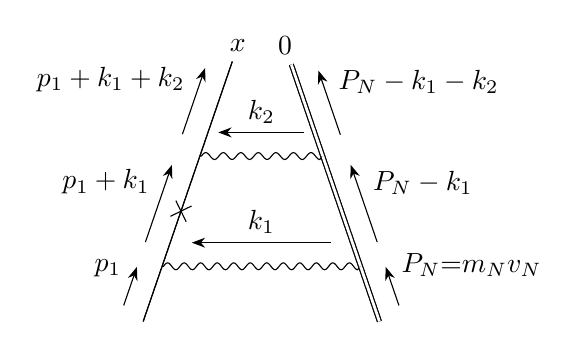
\begin{tikzpicture}[baseline=($(p1)!0.5!(x)$)]
		\begin{feynman}
		\vertex (p1);
		\vertex[right=3cm of p1] (p2);
		\vertex at ($(p1)!0.4!(p2)+(0,3.5cm)$) (x) {$x$};
		\vertex at ($(p1)!0.6!(p2)+(0,3.5cm)$) (0) {$0$};
		\vertex at ($(p1)!0.2!(x)$) (y1);
		\vertex at ($(p2)!0.2!(0)$) (z1);
		\vertex at ($(p1)!0.6!(x)$) (y2);
		\vertex at ($(p2)!0.6!(0)$) (z2);
		%
		\diagram* {
		  (p1) -- [] (x);
		  (p2) -- [double distance=1pt] (0);
		  (y1) -- [photon,rmomentum=$k_1$] (z1);
		  (y2) -- [photon,rmomentum=$k_2$] (z2);
		  (p1) -- [momentum=\(p_{1}\)] (y1);
		  (p2) -- [momentum'=$P_{N}\text{=}m_{N}v_{N}$,double distance=1pt] (z1);
		  (y1) -- [momentum=\(p_{1}+k_1\),insertion=0.5] (y2);
		  (z1) -- [momentum'=\(P_{N}-k_1\),double distance=1pt] (z2);
		  (y2) -- [momentum=\(p_{1}+k_1+k_2\)] (x);
		  (z2) -- [momentum'=\(P_{N}-k_1-k_2\),double distance=1pt] (0);
		};
		\end{feynman}
	  \end{tikzpicture}-
	  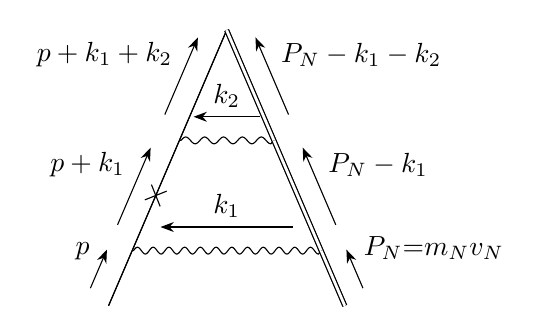
\begin{tikzpicture}[baseline=($(p1)!0.5!(x)$)]
		\begin{feynman}
			\vertex (p1);
			\vertex[right=3cm of p1] (p2);
			\vertex at ($(p1)!0.5!(p2)+(0,3.5cm)$) (x) ;
			\vertex at ($(p1)!0.2!(x)$) (y1);
			\vertex at ($(p2)!0.2!(x)$) (z1);
			\vertex at ($(p1)!0.6!(x)$) (y2);
			\vertex at ($(p2)!0.6!(x)$) (z2);
			\vertex at ($(y1)!0.5!(z1)$) (t);
			%
			\diagram* {
			(p1) -- [] (x);
			(p2) -- [double distance=1pt] (x);
			(y1) -- [photon,rmomentum=$k_1$] (z1);
			(y2) -- [photon,rmomentum=$k_2$] (z2);
			(p1) -- [momentum=\(p\)] (y1);
			(p2) -- [momentum'=$P_{N}\text{=}m_{N}v_{N}$,double distance=1pt] (z1);
			(y1) -- [momentum=\(p+k_1\),insertion=0.5] (y2);
			(z1) -- [momentum'=\(P_{N}-k_1\),double distance=1pt] (z2);
			(y2) -- [momentum=\(p+k_1+k_2\)] (x);
			(z2) -- [momentum'=\(P_{N}-k_1-k_2\),double distance=1pt] (x);
			};
		\end{feynman}
	\end{tikzpicture}\\
	=&4m^2\mu^{2\epsilon}Z^2e^4
	\int\frac{\dd^3\vb{k_1}}{(2\pi)^3}\frac{\dd^3\vb{k_2}}{(2\pi)^3}\bqty{e^{-i\vb{k}_2\cdot\vb{x}}-1}\frac{1}{\vb{\abs{k_1-p}}^2}\frac{1}{\vb{\abs{k_2-k_1}}^2}\frac{\vb{\abs{k_1}}^4/4m^2}{[\vb{\abs{k_1}}^2-2mE]^2}\frac{1}{\vb{\abs{k_2}}^2-2mE}
\end{align*}

\begin{appendices}
	\section{Useful formulas in Feynman integrals}
	Feynman parametrization used here is
	\begin{align}
		\frac{1}{\prod A_i^{d_i}}=\int\prod \dd x_i \delta(\sum x_i-1)\frac{\prod x_i^{d_i-1}}{\bqty{\sum x_iA_i}^{\sum d_i}}\frac{\Gamma(\sum d_i)}{\prod\Gamma(d_i)}
		\label{FEYNMANPARA}
	\end{align}
	Schwinger parametrization will also be useful
	\begin{align}
		\frac{1}{A^n}=\frac{1}{\Gamma{(n)}}\int_0^\infty\dd z z^{n-1}e^{-zA}
	\end{align}
	For arbitary one loop diagram of the following form, we have
	\begin{subequations} \label{1loopgamma}
		\begin{align}
			\int\frac{\dd^dk}{(2\pi)^d}\frac{k^{2\b}}{(k^2+\Delta)^n}
			  & =\frac{1}{(4\pi)^{n-\b}}\frac{\Gamma(\b+d/2)}{\Gamma(d/2)}\frac{\Gamma(n-\b-d/2)}{\Gamma(n)}\pqty{\frac{4\pi}{\Delta}}^{n-\b-d/2} \\
			  & =\frac{1}{(4\pi)^{d/2}}\frac{\Gamma(\b+d/2)}{\Gamma(d/2)}\frac{\Gamma(n-\b-d/2)}{\Gamma(n)}\pqty{\frac{1}{\Delta}}^{n-\b-d/2}
		\end{align}
	\end{subequations}
	where $\frac{1}{(4\pi)^{d/2}}$ often appears as $2^{-d}\pi^{-d/2}$.
	%  For two loop diagrams of this form ($\epsilon=3-d$)
	%  \begin{align}
	%	\mu^{-4\epsilon}\int\frac{\dd^d\vb{k}_1}{(2\pi)^d}\frac{\dd^d\vb{k}_2}{(2\pi)^d}\frac{1}{\vb{(k_1-a)}^2}\frac{1}{\vb{(k_2-k_1)}^2}\frac{\vbk_1^{2\a}}{(\vb{k}_1^2-c)^m}\frac{\vbk_2^{2\b}}{(\vb{k}_2^2-d)^n}
	%	\label{int}
	%  \end{align}
	%  The integral is evaluated to
	%  \begin{align*}
	%	&\mu^{-4\epsilon}\int_0^1\prod_{i=1}^2\dd x_i\delta(\sum x_i-1)\prod x_i^{d_i-1}\frac{\Gamma(n+1)}{\Gamma(n)}\frac{1}{(4\pi)^{n+1-\b}}\frac{\Gamma(\b+d/2)}{\Gamma(d/2)}\frac{\Gamma(n+1-\b-d/2)}{\Gamma(n+1)}\pqty{\frac{4\pi}{\a(x_i)}}^{n+1-\b-d/2}
	%	\\&\int\frac{\dd^d\vb{k}_1}{(2\pi)^d}\frac{1}{\vb{(k_1-a)}^2}\frac{\vbk_1^{2\a}}{(\vb{k}_1^2-c)^m}\frac{1}{(\vb{k}_1-\Delta_2)^{n+1-\b-d/2}}\\
	%	=&\mu^{-4\epsilon}\int_0^1\prod_{i=1}^2\dd x_i\delta(\sum x_i-1)\prod x_i^{d_i-1}\frac{1}{(4\pi)^{n+1-\b}}\frac{\Gamma(\b+d/2)}{\Gamma(d/2)}\frac{\Gamma(n+1-\b-d/2)}{\Gamma(n)}\pqty{\frac{4\pi}{\a(x_i)}}^{n+1-\b-d/2}\int_0^1\prod_{i=1}^3\dd y_j\delta(\sum y_j-1)
	%	\\&\prod y_j^{d_j-1}
	%	\frac{\Gamma(m+n+2-\b-d/2)}{\Gamma(m)\Gamma(n+1-\b-d/2)}\frac{1}{(4\pi)^{m+n+2-\a-\b-d/2}}\frac{\Gamma(\a+d/2)}{\Gamma(d/2)}\frac{\Gamma(m+n+2-\a-\b-d)}{\Gamma(m+n+2-\b-d/2)}\pqty{\frac{4\pi}{\Delta_1}}^{m+n+2-\a-\b-d}
	%	\\
	%	=&\mu^{-4\epsilon}\int_0^1\prod_{i=1}^2\dd x_i\delta(\sum x_i-1)\prod x_i^{d_i-1}\frac{1}{(4\pi)^{d}}\frac{\Gamma(\b+d/2)}{\Gamma(d/2)}\frac{1}{\Gamma(n)}\pqty{\frac{1}{\a(x_i)}}^{n+1-\b-d/2}
	%	\\&\int_0^1\prod_{i=1}^3\dd y_j\delta(\sum y_j-1)\prod y_j^{d_j-1}\frac{\Gamma(\a+d/2)}{\Gamma(d/2)}\frac{\Gamma(m+n+2-\a-\b-d)}{\Gamma(m)}\pqty{\frac{1}{\Delta_1}}^{m+n+2-\a-\b-d}
	% \end{align*}<++>
	\section{Contour Integral}
	If the nucleus is put on-shell, integral with the structure of the form
	\begin{align*}
		\int[dk_1][dk_2]f(\vb{k}_1,\vb{k}_2)\frac{1}{-k_1^0-k_2^0+i\epsilon}\frac{1}{-k_1^0+i\epsilon}\frac{1}{[E+k_1^0-\vb{V}_2+i\epsilon]^m}\frac{1}{[E+k_1^0+k_2^0-\vb{V}_2+i\epsilon]^n}
	\end{align*}
	will always produce
	\begin{align*}
		\int\frac{\dd^3\vb{k_1}}{(2\pi)^3}\frac{\dd^3\vb{k_2}}{(2\pi)^3}f(\vb{k}_1,\vb{k}_2)\frac{1}{[E-\vb{V}_1+2i\epsilon]^m}\frac{1}{[E-\vb{V}_2+2i\epsilon]^n}
	\end{align*}
	with $k_1^0$ and $k_2^0$ goes to zero.

	If the nucleus is slightly off-shell by $k$, there'll be a slight shift of energy in the non-relativistic propagators
	\begin{align*}
		&\int[dk_1][dk_2]f(\vb{k}_1,\vb{k}_2)\frac{1}{-k_1^0-k_2^0+k^0+i\epsilon}\frac{1}{-k_1^0+k^0+i\epsilon}\frac{1}{[E+k_1^0-\vb{V}_2+i\epsilon]^m}\frac{1}{[E+k_1^0+k_2^0-\vb{V}_2+i\epsilon]^n}\\
		=&\int\frac{\dd^3\vb{k_1}}{(2\pi)^3}\frac{\dd^3\vb{k_2}}{(2\pi)^3}f(\vb{k}_1,\vb{k}_2)\frac{1}{[E+k^0-\vb{V}_1+2i\epsilon]^m}\frac{1}{[E+k^0-\vb{V}_2+2i\epsilon]^n}
	\end{align*}
	one example is this Green function
	\begin{align*}
		&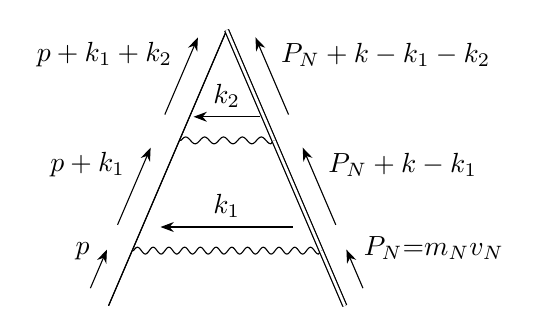
\begin{tikzpicture}[baseline=($(p1)!0.5!(x)$)]
			\begin{feynman}
				\vertex (p1);
				\vertex[right=3cm of p1] (p2);
				\vertex at ($(p1)!0.5!(p2)+(0,3.5cm)$) (x) ;
				\vertex at ($(p1)!0.2!(x)$) (y1);
				\vertex at ($(p2)!0.2!(x)$) (z1);
				\vertex at ($(p1)!0.6!(x)$) (y2);
				\vertex at ($(p2)!0.6!(x)$) (z2);
				%
				\diagram* {
				(p1) -- [] (x);
				(p2) -- [double distance=1pt] (x);
				(y1) -- [photon,rmomentum=$k_1$] (z1);
				(y2) -- [photon,rmomentum=$k_2$] (z2);
				(p1) -- [momentum=\(p\)] (y1);
				(p2) -- [momentum'=$P_{N}\text{=}m_{N}v_{N}$,double distance=1pt] (z1);
				(y1) -- [momentum=\(p+k_1\)] (y2);
				(z1) -- [momentum'=\(P_{N}+k-k_1\),double distance=1pt] (z2);
				(y2) -- [momentum=\(p+k_1+k_2\)] (x);
				(z2) -- [momentum'=\(P_{N}+k-k_1-k_2\),double distance=1pt] (x);
				};
			\end{feynman}
		\end{tikzpicture}
	\end{align*}
\end{appendices}

\bibliographystyle{phaip}

\bibliography{QM-OPE}

\end{document}
